\documentclass{article}

\usepackage[preprint]{neurips_2024}

\usepackage[utf8]{inputenc}
\usepackage[T1]{fontenc}
\usepackage{hyperref}
\usepackage{url}
\usepackage{booktabs}
\usepackage{amsfonts}
\usepackage{amsmath}
\usepackage{nicefrac}
\usepackage{microtype}
\usepackage{xcolor}
\usepackage{graphicx}

\title{StreamLip: Streaming Lip-to-Speech Synthesis via Joint Text-Audio Decoding with Flow Matching}

\author{%
  Changxun Pan \\
  \texttt{2024011323} \\
  \And
  Anqiao Fu \\
  \texttt{2024010753} \\
  \And
  Zihan Guo \\
  \texttt{2024011317} \\
}

\begin{document}
\maketitle

\begin{abstract}
We propose \textbf{StreamLip}, the first streaming lip-to-speech (L2S) synthesis system that generates intelligible speech from silent video in real time. Our model jointly decodes text tokens and audio features within a unified autoregressive framework: a causal Transformer backbone with a look-ahead window predicts text tokens via autoregressive cross-entropy, while a lightweight flow matching head generates audio codec latents conditioned on both the visual features and the predicted text hidden states. This design addresses the fundamental viseme-to-phoneme ambiguity in L2S through an internal language model prior, without requiring an external lip-reading module at inference time. We plan to evaluate on LRS3 and demonstrate that our streaming approach, despite operating under strict causal constraints with only 200\,ms of future context, can produce speech of reasonable intelligibility and naturalness.
\end{abstract}

%======================================================================
\section{Introduction}
%======================================================================

Lip-to-speech (L2S) synthesis aims to generate natural speech from silent talking face videos. This technology has potential applications in assistive communication for individuals with speech impairments, bandwidth-efficient video conferencing, and privacy-preserving voice reconstruction. Recent advances in diffusion and flow matching models have significantly improved the quality of L2S systems. LipVoicer~\cite{lipvoicer} demonstrated that text guidance is essential for resolving the one-to-many viseme-to-phoneme mapping, reducing word error rate (WER) from 86\% to 21\% on LRS3. V2SFlow~\cite{v2sflow} introduced rectified flow matching to L2S and achieved naturalness surpassing ground truth. Most recently, SLD-L2S~\cite{sldl2s} established a new state of the art by operating in neural audio codec latent spaces.

However, all existing L2S methods share a critical limitation: \textbf{they operate offline}, requiring access to the entire video before generating any speech. This precludes real-time applications where low-latency speech output is necessary---such as live assistive communication devices that must maintain natural conversational rhythm ($\leq$200\,ms latency).

Meanwhile, adjacent fields have made progress on streaming generation. SoundReactor~\cite{soundreactor} proposed the first frame-level online video-to-audio generator using a causal autoregressive (AR) Transformer with a diffusion head, achieving 26\,ms per-frame latency on game audio. Moshi~\cite{moshi} introduced the \textit{Inner Monologue} mechanism for full-duplex spoken dialogue, where predicting time-aligned text tokens before audio tokens serves as a semantic scaffold that improves speech quality. UniVoice~\cite{univoice} unified AR-based ASR and flow-matching-based TTS within a single language model, demonstrating that discrete text prediction and continuous audio generation can coexist through careful loss balancing ($\lambda{=}0.005$) and dual attention mechanisms.

\textbf{Our key observation} is that these three ideas---streaming causal generation (SoundReactor), text-as-semantic-prior (Moshi), and AR+FM joint training (UniVoice)---can be synthesized into a unified framework for streaming L2S.  We propose \textbf{StreamLip}, which makes three contributions:

\begin{enumerate}
    \item \textbf{First streaming L2S system.} We formulate L2S as a causal, chunk-based generation problem with a 200\,ms look-ahead window, enabling real-time speech synthesis from video.
    \item \textbf{Joint text-audio decoding.} A single AR backbone simultaneously predicts text tokens (providing a language model prior to resolve viseme ambiguity) and conditions a flow matching head for audio generation, eliminating the need for an external lip-reading module.
    \item \textbf{AR + flow matching co-training.} We adapt techniques from multi-task learning---stop-gradient isolation and scheduled corruption---to stably train the discrete text branch and continuous audio branch end-to-end.
\end{enumerate}

\begin{figure}[htbp]
  \centering
  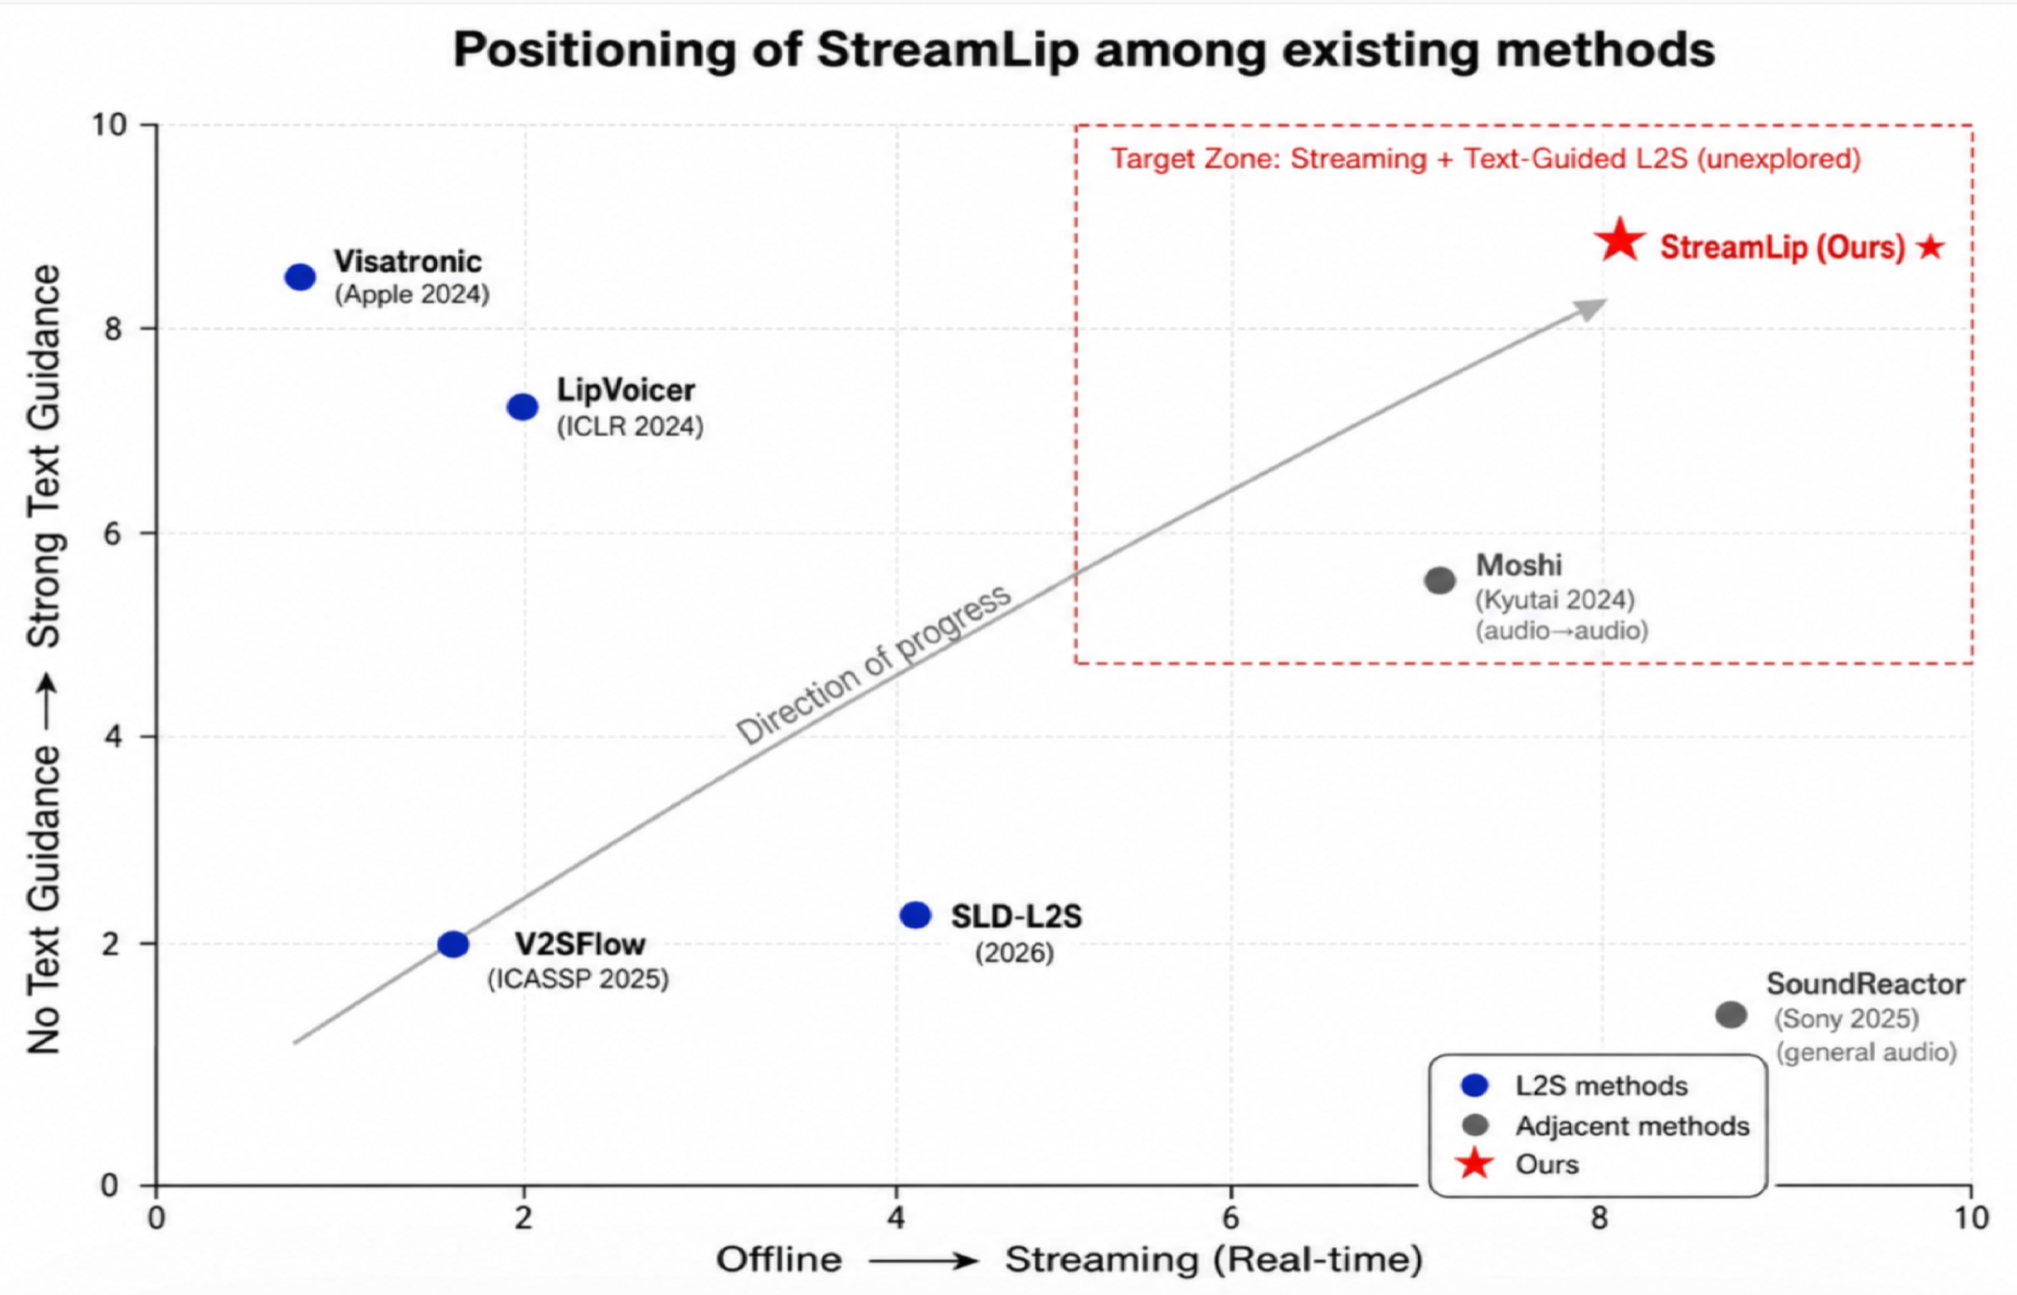
\includegraphics[width=0.8\textwidth]{fig_position.png}
  \caption{Positioning of StreamLip among existing L2S and related generative methods. Our approach targets the unexplored intersection of real-time streaming constraints and strong text guidance.}
  \label{fig:position}
\end{figure}

%======================================================================
\section{Goal of Achievement}
%======================================================================

We aim to demonstrate a working streaming L2S system with the following measurable targets on the LRS3-TED benchmark~\cite{lrs3}:

\begin{itemize}
    \item \textbf{Intelligibility}: WER $\leq$ 40\% (measured via a pre-trained ASR model). For reference, LipVoicer~\cite{lipvoicer} (offline, with external VSR) achieves 21\%; V2SFlow~\cite{v2sflow} (offline, no text) achieves 28.5\%.
    \item \textbf{Naturalness}: UTMOS $\geq$ 3.0 (ground truth is 3.52). V2SFlow achieves 3.78 in offline mode.
    \item \textbf{Latency}: End-to-end latency $\leq$ 250\,ms (200\,ms look-ahead + $\leq$50\,ms compute). Moshi operates at $\sim$200\,ms for comparison.
    \item \textbf{Ablation evidence}: Demonstrate through controlled experiments that (a) the text branch improves WER over a text-free baseline, and (b) the look-ahead window improves quality over a purely causal baseline.
\end{itemize}

We consider WER $\leq$ 40\% a realistic target because: (1) the AR text head has access to full past context plus language model priors, which partially compensates for the limited visual window; (2) many WER ``errors'' on homophones (buy/by, their/there) produce acoustically identical speech.

%======================================================================
\section{Methods}
%======================================================================

\subsection{Problem Formulation}

Given a silent video sequence $V = \{V_1, \ldots, V_n\}$ at 25\,fps, we generate speech audio in a streaming fashion. At each time step $i$, the model can observe $V_{\leq i+\Delta}$ where $\Delta{=}5$ frames (200\,ms look-ahead) and all previously generated audio. The output is a sequence of audio chunks, each corresponding to one video frame's worth of speech ($\sim$40\,ms).

Formally, we factorize the joint distribution as:
\begin{equation}
    p(\mathbf{a}_{1:n}, \mathbf{w}_{1:n} \mid V_{1:n}) = \prod_{i=1}^{n} p(\mathbf{w}_i \mid V_{\leq i+\Delta}, \mathbf{w}_{<i}) \cdot p(\mathbf{a}_i \mid V_{\leq i+\Delta}, \mathbf{w}_{\leq i}, \mathbf{a}_{<i})
\end{equation}
where $\mathbf{w}_i$ is the text token at step $i$ (predicted autoregressively) and $\mathbf{a}_i$ is the audio latent at step $i$ (generated via flow matching conditioned on $\mathbf{w}_{\leq i}$ and $V_{\leq i+\Delta}$). Text is predicted \textit{before} audio at each step, following Moshi's Inner Monologue principle~\cite{moshi}.

\subsection{Architecture}

The system consists of four components (Figure~\ref{fig:arch}):

\begin{figure}[htbp]
  \centering
  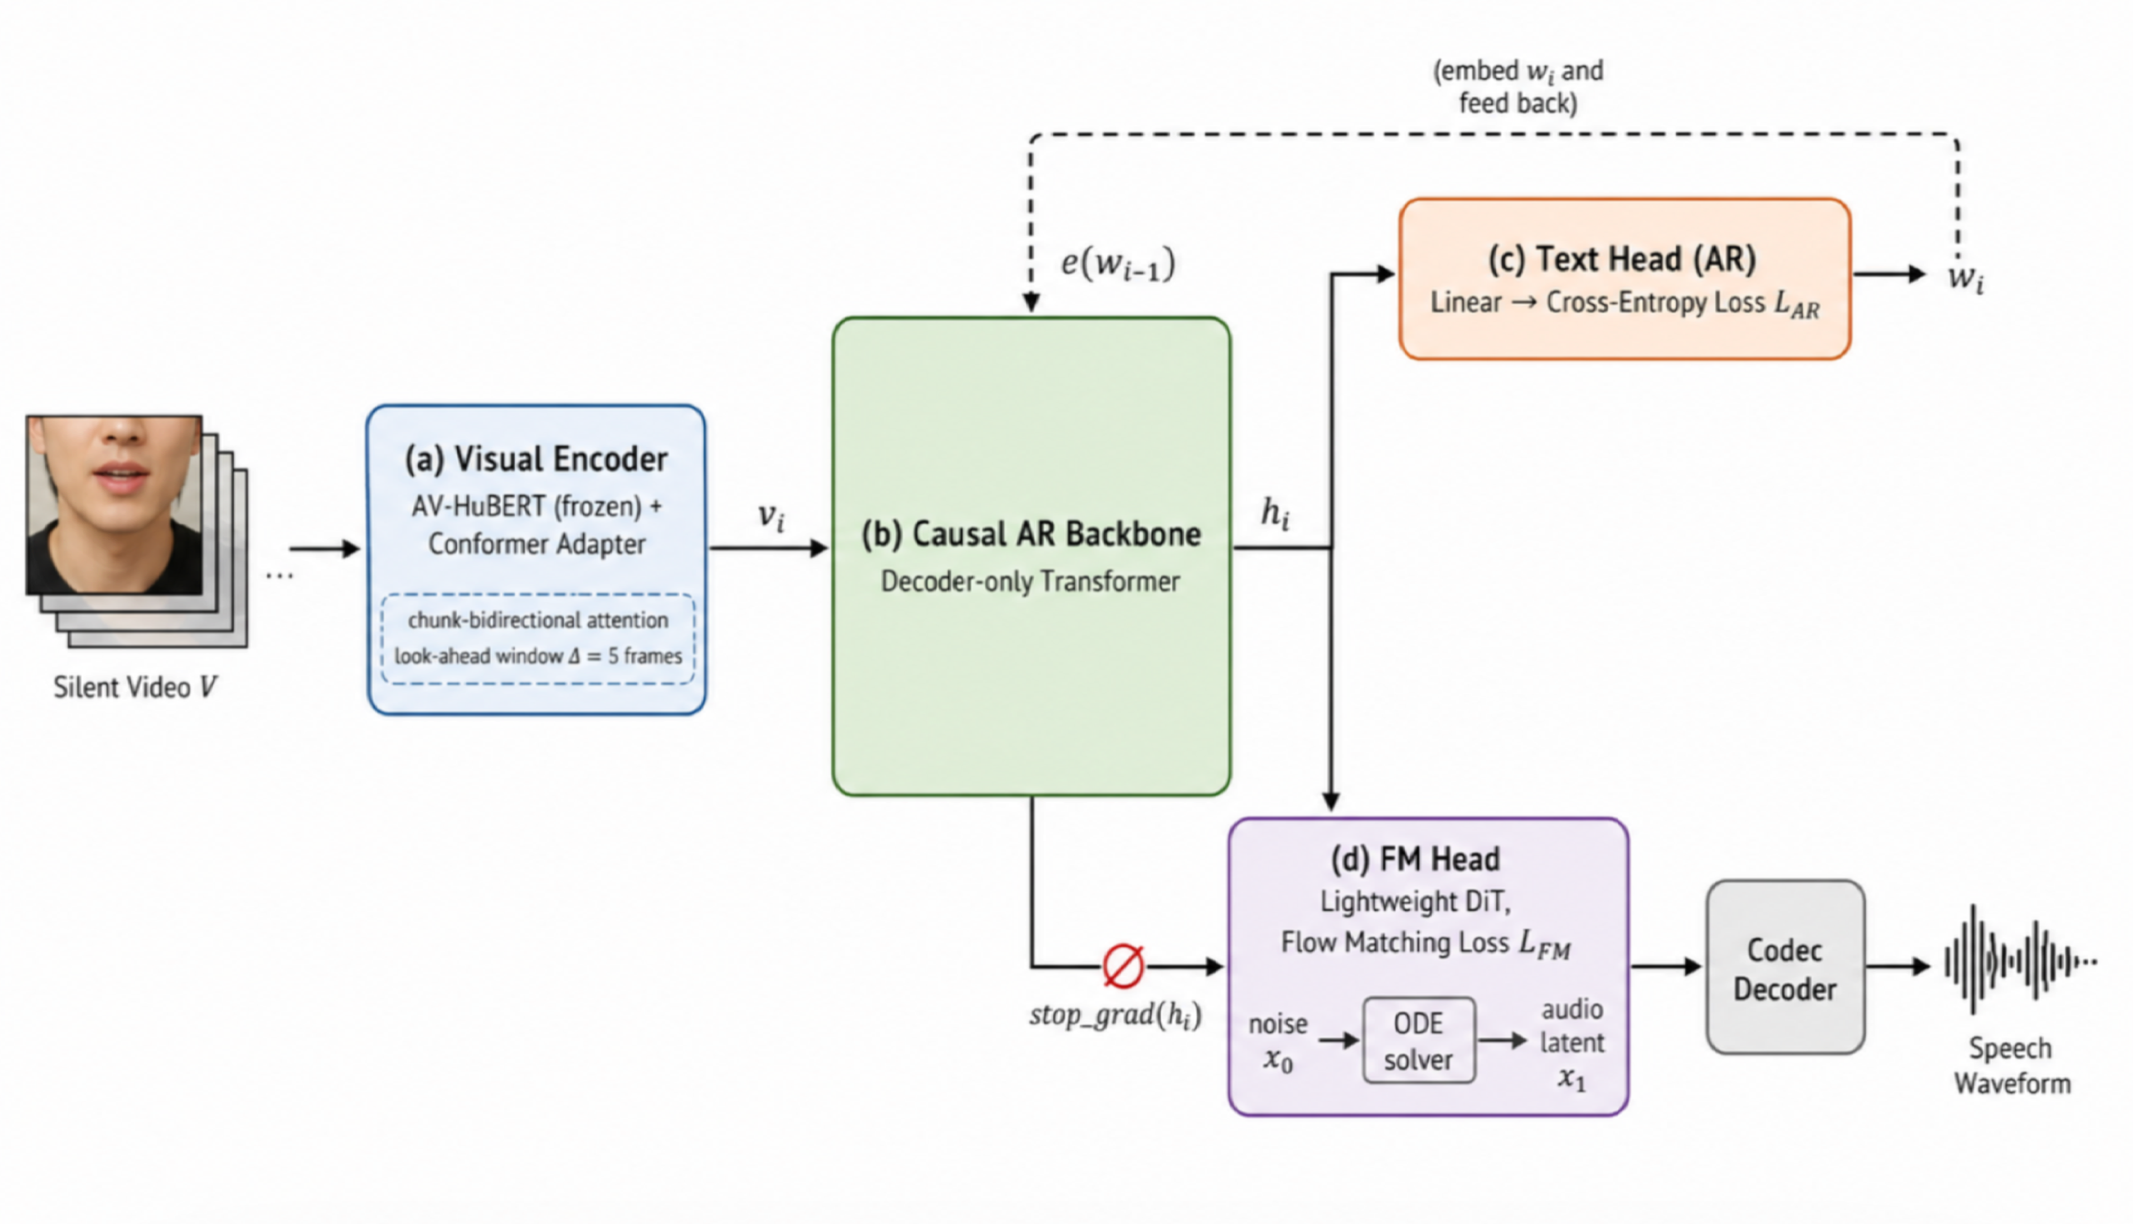
\includegraphics[width=\textwidth]{fig_arch.png}
  \caption{The StreamLip architecture. A causal AR backbone processes visual features and predicts text tokens. A lightweight flow matching head, conditioned on the text hidden states (with stop-gradient isolation), generates audio codec latents.}
  \label{fig:arch}
\end{figure}

\paragraph{(a) Visual Encoder.} We use a frozen AV-HuBERT (Large)~\cite{avhubert} to extract visual features from cropped lip regions. AV-HuBERT outputs 1024-dim features at 25\,Hz. To incorporate the look-ahead window, we apply chunk-level bidirectional self-attention: within each chunk of $1{+}\Delta$ frames, attention is bidirectional; across chunks, it is causal. A lightweight Conformer~\cite{conformer} adapter projects features to the backbone dimension.

\paragraph{(b) Causal AR Backbone.} A decoder-only Transformer processes the interleaved sequence of visual features and token embeddings. At each time step $i$, the backbone receives the visual feature $\mathbf{v}_i$ (with look-ahead context) and the previous text token embedding $\mathbf{e}(\mathbf{w}_{i-1})$, producing a hidden state $\mathbf{h}_i$.

\paragraph{(c) Text Head (AR).} A linear projection maps $\mathbf{h}_i$ to logits over the text vocabulary, trained with cross-entropy loss:
\begin{equation}
    \mathcal{L}_{\text{AR}} = -\sum_{i=1}^{n} \log p(\mathbf{w}_i \mid \mathbf{h}_i)
\end{equation}
During training, we use ground-truth text tokens from forced alignment. During inference, the text head autoregressively samples tokens. Critically, we pass the \textit{continuous hidden state} $\mathbf{h}_i$ (not the discrete sampled token) to the FM head, preserving uncertainty information.

\paragraph{(d) Flow Matching Head (FM).} A lightweight DiT~\cite{dit} (4--6 layers) generates audio codec latents conditioned on $\mathbf{h}_i$ (which encodes both visual and textual information). Following SLD-L2S~\cite{sldl2s}, we operate in the continuous latent space of a pre-trained audio codec (e.g., X-Codec or Mimi~\cite{moshi}).

The FM head models the vector field from noise $\mathbf{x}_0 \sim \mathcal{N}(0, I)$ to target audio latent $\mathbf{x}_1$:
\begin{equation}
    \mathcal{L}_{\text{FM}} = \mathbb{E}_{t, \mathbf{x}_0, \mathbf{x}_1} \left\| v_\theta(\mathbf{x}_t, t \mid \mathbf{h}_i) - (\mathbf{x}_1 - \mathbf{x}_0) \right\|^2, \quad \mathbf{x}_t = (1{-}t)\mathbf{x}_0 + t\,\mathbf{x}_1
\end{equation}
where $t \sim \mathcal{U}(0,1)$ and $\mathbf{h}_i$ is injected via adaLN-Zero conditioning~\cite{dit}. At inference, we use an Euler solver with 10 steps and classifier-free guidance~\cite{cfg}.

\subsection{Training Strategy}

\paragraph{Joint loss.} The total loss combines both branches:
\begin{equation}
    \mathcal{L} = \mathcal{L}_{\text{FM}}(\theta_{\text{fm}} \mid \texttt{stop\_grad}(\mathbf{h}_i)) + \lambda \cdot \mathcal{L}_{\text{AR}}(\theta_{\text{backbone}}, \theta_{\text{text}})
\end{equation}
The FM loss gradient does not flow back through the backbone (stop-gradient), preventing the continuous audio gradients from destabilizing the discrete text predictions. Only $\mathcal{L}_{\text{AR}}$ updates the backbone. We set $\lambda{=}1.0$ for the AR branch since it is the sole driver of backbone learning.

\paragraph{Scheduled corruption.} To prevent the FM head from over-relying on the text hidden states (which will be noisier at inference due to autoregressive error accumulation), we corrupt the text condition during training: with probability $p_{\text{mask}}{=}0.1$, we replace $\mathbf{h}_i$ with a zero vector; with probability $p_{\text{noise}}{=}0.05$, we add Gaussian noise to $\mathbf{h}_i$. This trains the FM head to gracefully degrade when text information is unreliable, falling back on visual features and acoustic continuity.

\paragraph{Training phases.}
\begin{enumerate}
    \item \textbf{Phase 1} (Backbone + Text Head): Train the visual encoder adapter and AR backbone on the lip-reading task only ($\mathcal{L}_{\text{AR}}$), warm-starting from a pre-trained LM if available. This produces a capable visual-conditioned language model.
    \item \textbf{Phase 2} (Joint): Attach the FM head and train jointly with stop-gradient. The FM head learns to generate audio conditioned on the now-frozen-quality text hidden states.
\end{enumerate}

\subsection{Inference Pipeline}

At each time step $i$:
\begin{enumerate}
    \item Wait for frame $V_{i+\Delta}$ (200\,ms look-ahead).
    \item Encode $V_{[i-K, i+\Delta]}$ through the visual encoder with chunk-bidirectional attention.
    \item The AR backbone produces $\mathbf{h}_i$ and samples text token $\mathbf{w}_i$.
    \item The FM head generates audio latent $\mathbf{a}_i$ from noise, conditioned on $\mathbf{h}_i$, using 10-step Euler ODE.
    \item Decode $\mathbf{a}_i$ through the pre-trained codec decoder to produce a waveform chunk.
    \item Overlap-add with the previous chunk (50\,ms overlap + linear crossfade) for smooth output.
\end{enumerate}

\begin{figure}[htbp]
  \centering
  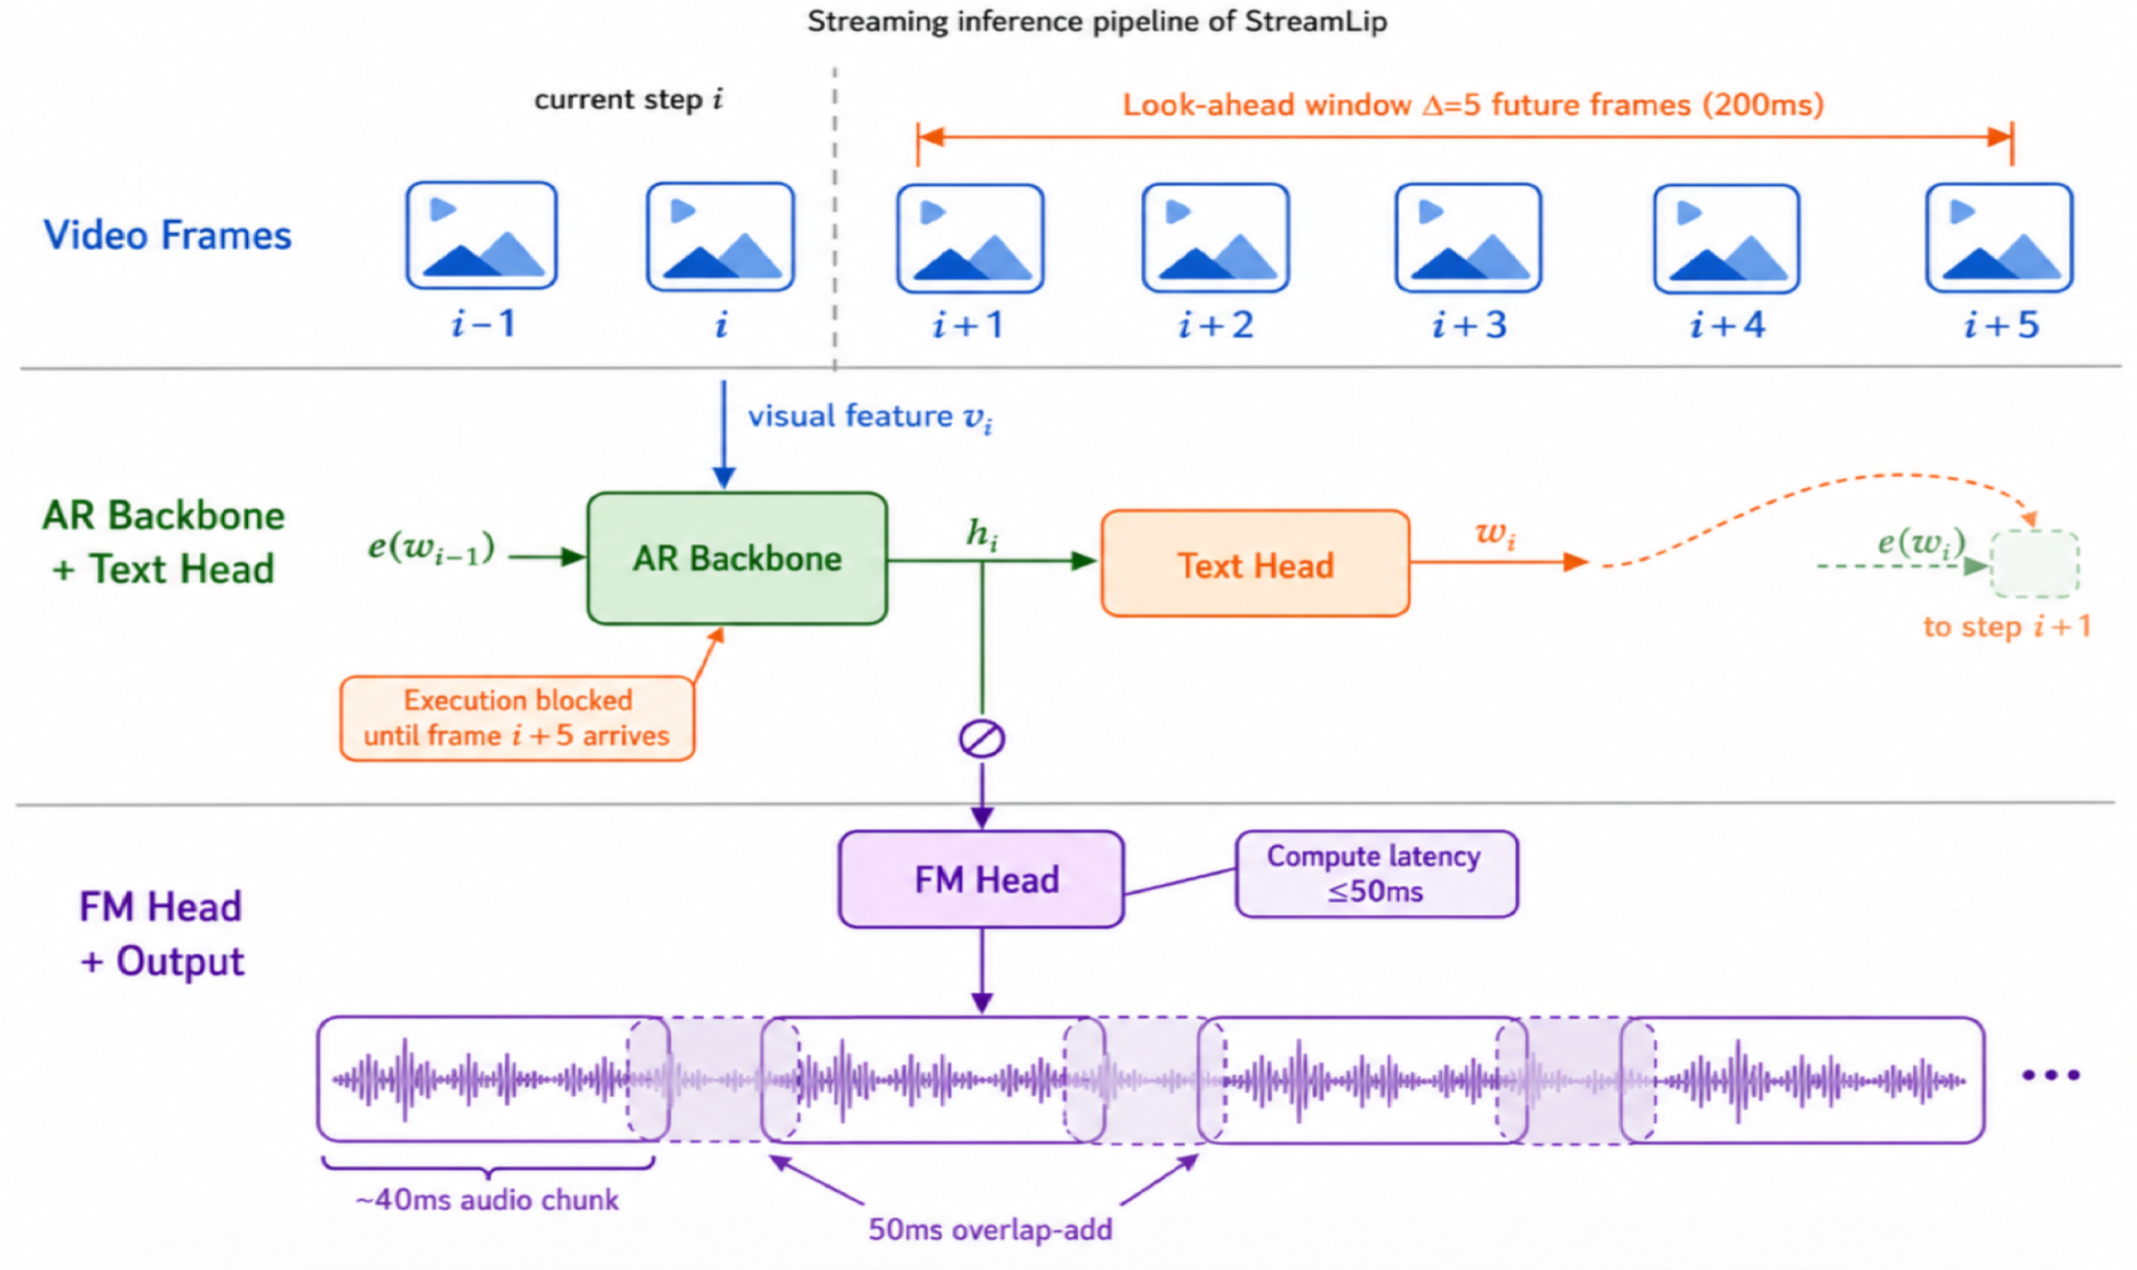
\includegraphics[width=\textwidth]{fig_timeline.png}
  \caption{Streaming inference pipeline. The model uses a 200\,ms look-ahead window. Text tokens are predicted autoregressively to build semantic context, while audio chunks are generated and crossfaded to produce continuous streaming speech with $\le$250\,ms latency.}
  \label{fig:timeline}
\end{figure}

\subsection{Evaluation Plan}

We evaluate on LRS3-TED~\cite{lrs3} with the following metrics:
\begin{itemize}
    \item \textbf{Intelligibility}: WER (via pre-trained ASR), SpeechBERTScore.
    \item \textbf{Quality}: UTMOS, PESQ.
    \item \textbf{Speaker similarity}: SECS (Speaker Embedding Cosine Similarity).
    \item \textbf{Lip sync}: LSE-C (Lip Sync Error - Confidence) via SyncNet.
    \item \textbf{Latency}: Per-frame waveform-level latency (ms).
\end{itemize}

Key ablations:
\begin{itemize}
    \item \textbf{StreamLip (full)} vs.\ \textbf{w/o text head}: Measures the contribution of the language model prior.
    \item \textbf{StreamLip (full)} vs.\ \textbf{w/o look-ahead}: Measures the contribution of the 200\,ms future context.
    \item \textbf{StreamLip (full)} vs.\ \textbf{w/ GT text}: Upper bound on text prior quality.
    \item \textbf{StreamLip (full)} vs.\ \textbf{Chunked V2SFlow}: Offline method constrained to same chunk size (fair baseline).
\end{itemize}

%======================================================================
\section{Timeline}
%======================================================================

\begin{table}[h]
\centering
\small
\begin{tabular}{@{}lll@{}}
\toprule
\textbf{Period} & \textbf{Milestone} & \textbf{Deliverable} \\
\midrule
Week 1 & Data prep \& baseline setup & Preprocessed LRS3, initial text head \\
Week 2 & AR backbone implementation & Streaming lip-reading prototype \\
Week 3 & FM head \& joint training & End-to-end L2S training pipeline \\
Week 4 & Evaluation \& writing & Final report \& poster \\
\bottomrule
\end{tabular}
\end{table}

%======================================================================
\section{Workload Distribution}
%======================================================================

\begin{table}[h]
\centering
\small
\begin{tabular}{@{}ll@{}}
\toprule
\textbf{Member} & \textbf{Responsibilities} \\
\midrule
Changxun Pan & FM head implementation; audio codec integration; evaluation pipeline \\
Anqiao Fu & Visual encoder integration; data pipeline; look-ahead windowing \\
Zihan Guo & Overall architecture design; AR backbone \& text head implementation \\
\midrule
All & Literature review; experimental analysis; report writing; poster \\
\bottomrule
\end{tabular}
\end{table}

\bibliographystyle{unsrt}
\bibliography{ref}

\end{document}
